% !TEX root = ../paper.tex

\section{Design}

The priority queue implementation by \citeauthor{calciu_adaptive_2014} exports the two operations \texttt{add()} and \texttt{removeMin()}. It is based on a skiplist which is split into two parts as it can be seen in figure~\ref{fig:pqe}. The elements in the skiplist are buckets having associated keys accessible via \texttt{bucket.key}. \texttt{RemoveMin()} and \texttt{add()} operations with small keys are served by the sequential part, while \texttt{add()} operations with keys over a certain threshold are executed on the parallel part. The last element of the sequential part is referred to as \texttt{lastSeq} \cite{calciu_adaptive_2014}.

\begin{figure}[htb]
	\centering
	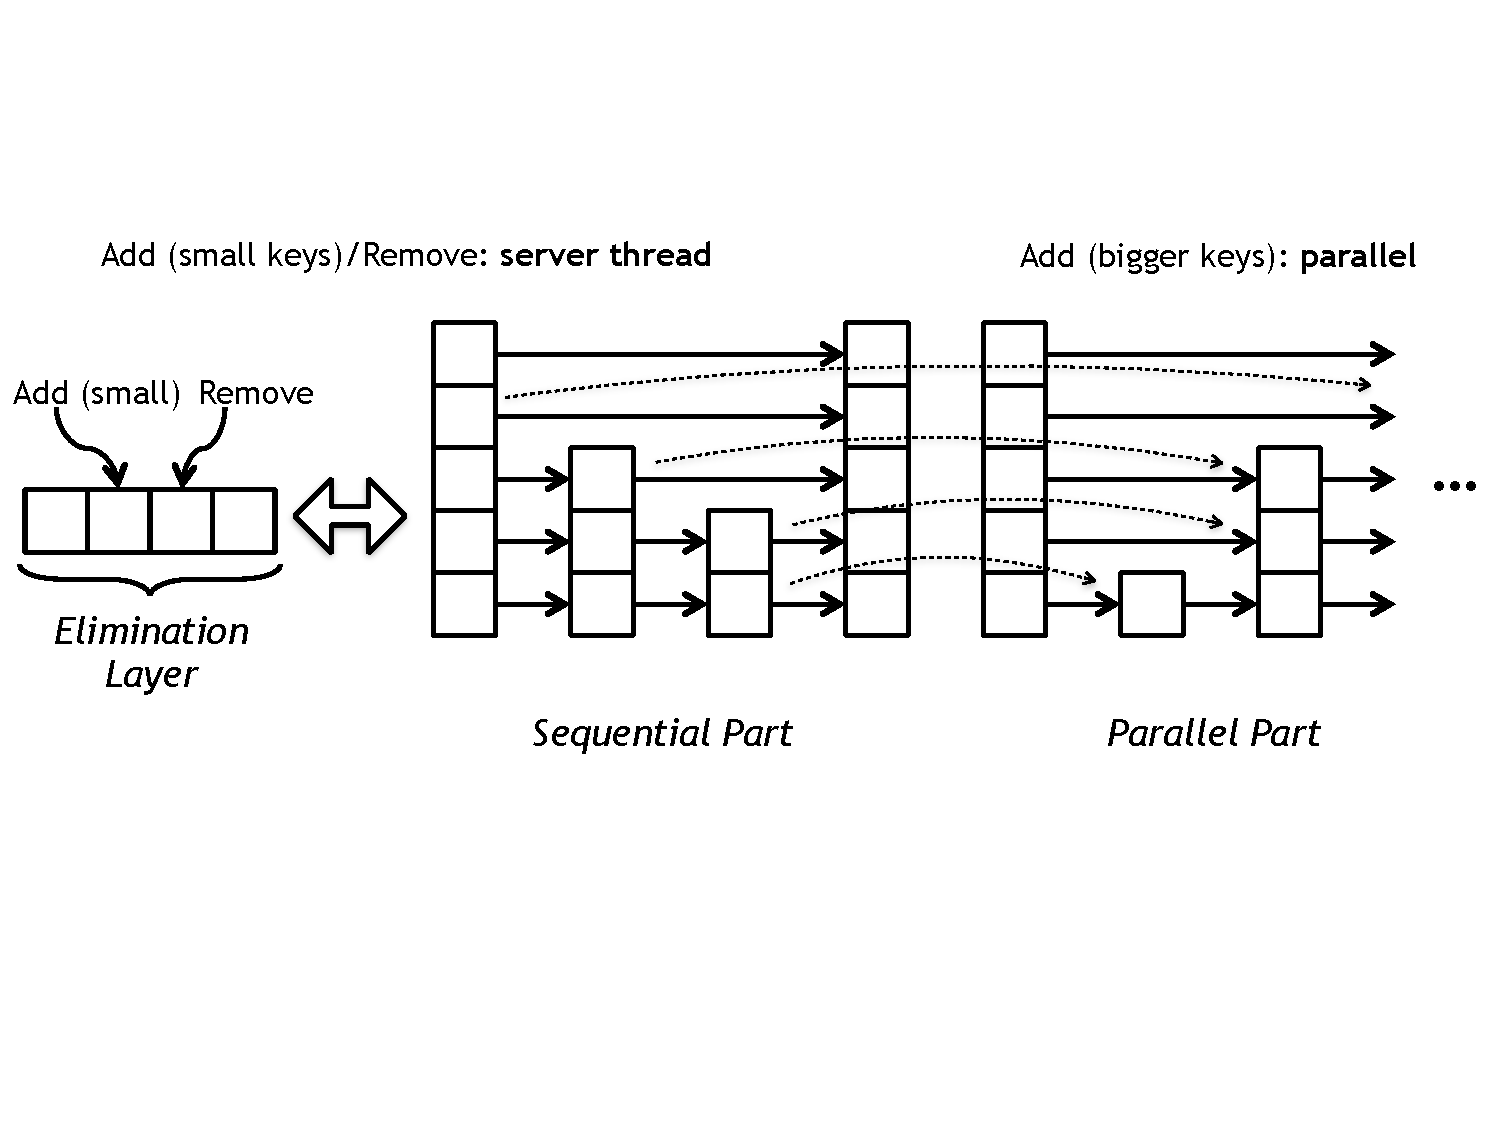
\includegraphics[width=0.9\textwidth]{graphics/pqe.pdf}
	\caption{Skiplist design \cite{calciu_adaptive_2014}.}
	\label{fig:pqe}
\end{figure}

\paragraph{Add()}

A thread executing \texttt{add($v$)} on the priority queue decides to insert the element concurrently into the parallel part if $v > \texttt{lastseq.key}$. Otherwise, the element is put into the elimination array as and add request. If the element becomes eligible for elimination ($v < \texttt{minValue}$) the operation can eliminate with any \texttt{removeMin()} occurring, otherwise the operation will be executed by the server thread \cite{calciu_adaptive_2014}.

\paragraph{RemoveMin()}

operations try to eliminate with an \texttt{add()} operation from the elimination array. If no operation is available, the thread writes a remove request to the array. It then gets either eliminated by a suitable \texttt{add()} operation or served by the server thread \cite{calciu_adaptive_2014}.

\subsection{Elimination and Combining}

Elimination allows operations to cancel each other out without accessing the shared datastructure. This reduces contention on the priority queue itself and therefore increases parallelism and scalability. The priority queue allows \texttt{removeMin()} operations to eliminate \texttt{add()} operations with keys smaller than \texttt{minValue} and vice versa. An array with a fixed size is used to store data the operations need to exchange \cite{calciu_adaptive_2014}.

\subsubsection{Elimination Array}

64 bit array slots are used to store a 32-bit value or one of the predefined opcodes as well as a unique stamp for every operation. Valid opcodes are: \texttt{EMPTY}, \texttt{REMREQ}, \texttt{INPROG}, and \texttt{TAKEN}. The values corresponding to these opcodes are not allowed to be used as values in the priority queue. These opcodes have following meaning:

\begin{description}
	\item[EMPTY] signals an unused slot of the elimination array.
	\item[REMREQ] is used by threads during a \texttt{removeMin()} operation to signal other threads the possibility to eliminate or instruct the server thread to remove an item from the priority queue.
	\item[INPROG] signals an adding thread that the server thread started to process the value that it wanted to add.
	\item[TAKEN] signals an adding thread that the value has been processed either by the server thread or a removing thread.
\end{description}

Other values stored in the elimination array are actual values being exchanged. The unique stamp also stored with the opcode/value is used for recognizing changes to the values stored in the elimination array and therefore ensuring linearizablity which will be covered in detail in section~\ref{sec:linearizablity}. This stamp is obtained by the thread ID and a thread-local operation counter \cite{calciu_adaptive_2014}.

\subsubsection{Operations and Elimination}

State transitions in the elimination array follow the state machine shown in figure~\ref{fig:combining-state}. Every slot is initially \texttt{EMPTY} with a stamp of 0. 

\begin{figure}[htb]
	\centering
	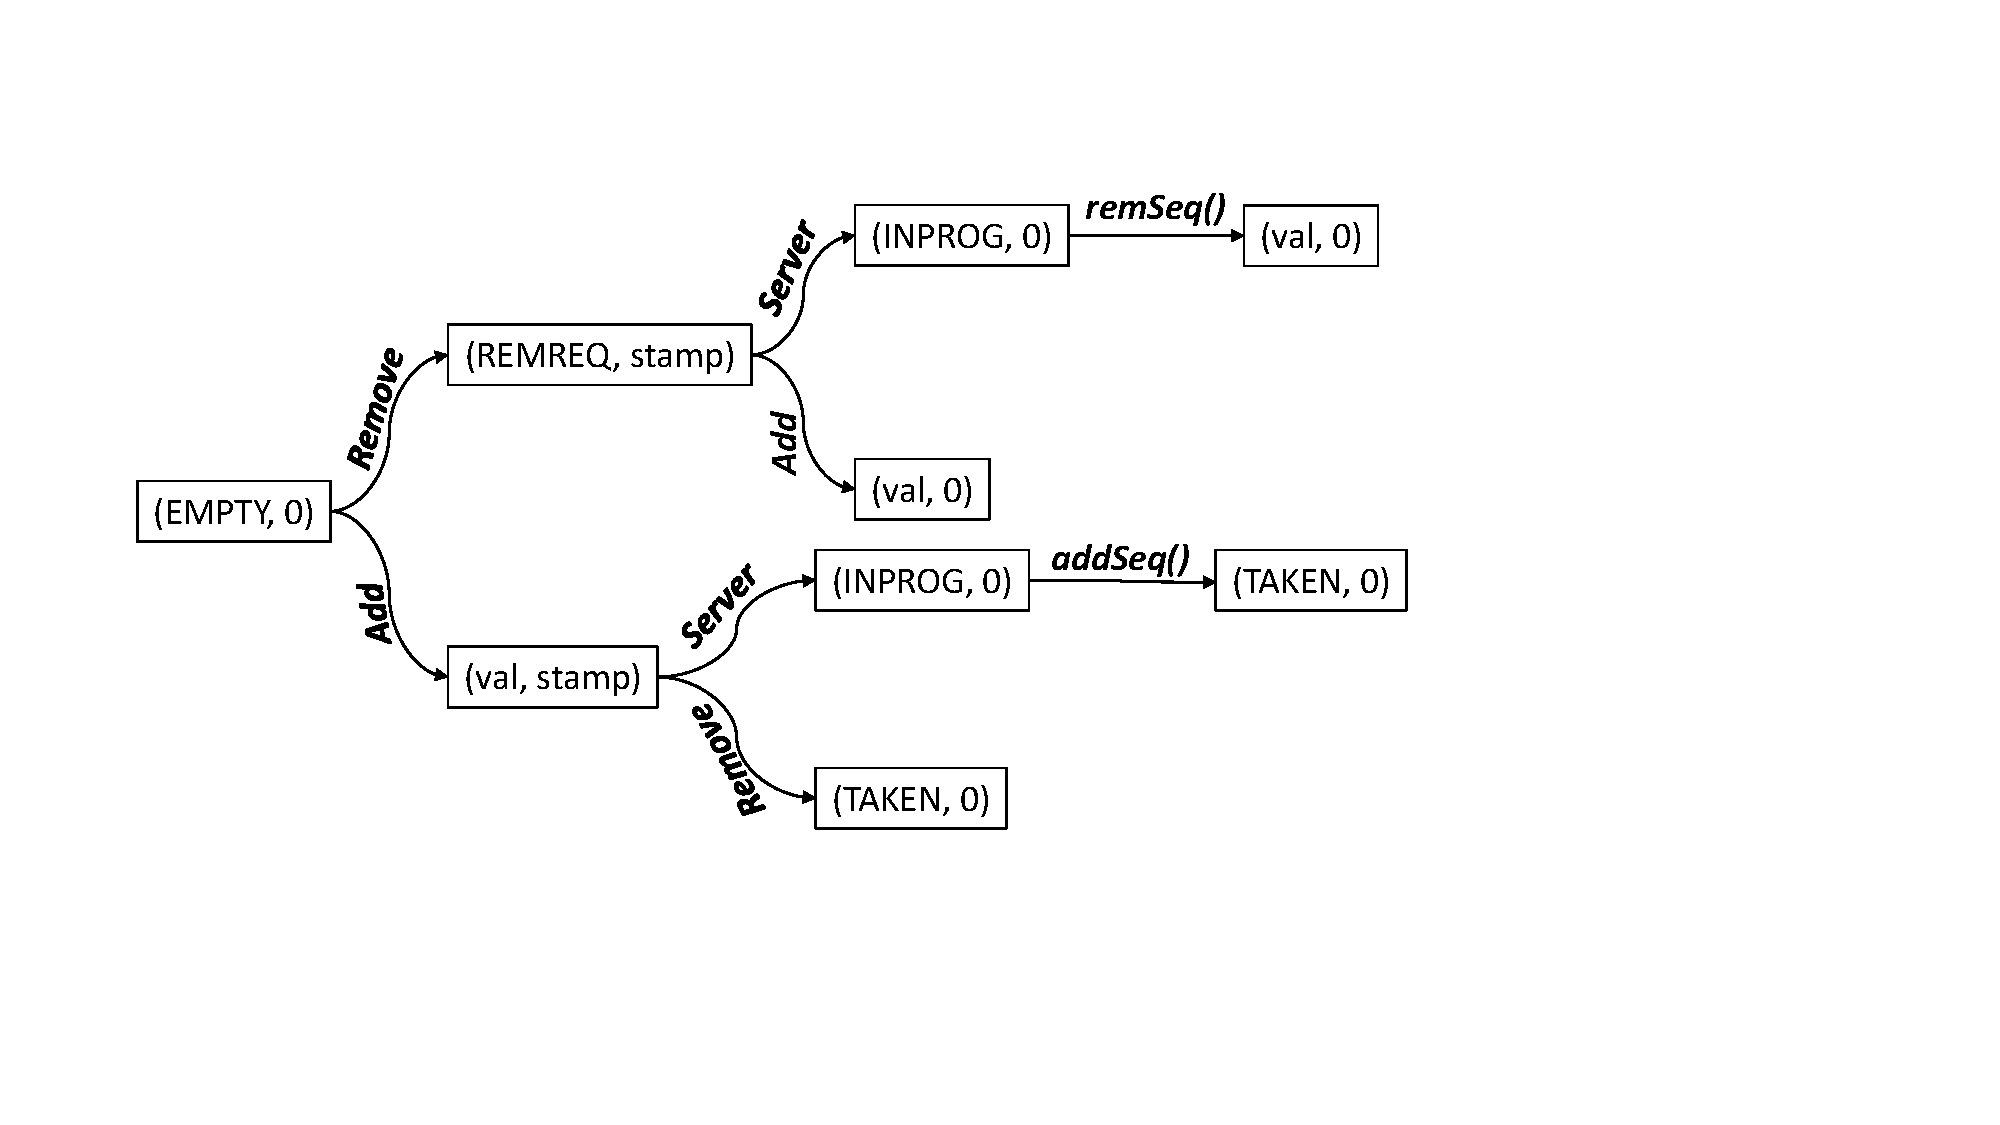
\includegraphics[width=0.9\textwidth]{graphics/combining-state.pdf}
	\caption{Elimination array state transitions \cite{calciu_adaptive_2014}.}
	\label{fig:combining-state}
\end{figure}

\paragraph{Add()} A thread trying to add a \texttt{key} (where $\texttt{key} < \texttt{minValue}$) iterates through all slots of the elimination array to find a \texttt{REMREQ} opcode. If it finds one and additionally $\texttt{key} < \texttt{minValue}$, the tread uses \texttt{CAS} to write its value including a stamp into this slot. If multiple attempts fail, the thread instead writes its value into a slot marked as \texttt{EMPTY} and waits for another or the server thread to use the value and change the opcode to \texttt{TAKEN} \cite{calciu_adaptive_2014}.

\paragraph{RemoveMin()} A thread removing an element from the priority queue iterates through the elimination array until it finds a value or an \texttt{EMPTY} slot in the elimination array. If the stamp of this value is greater than zero, it is checked whether the value is smaller than \texttt{minValue}, otherwise a non positive stamp indicates a value to respond to another \texttt{REMREQ}. In the case of the value being a current minimum of the priority queue the thread uses \texttt{CAS} to replace the value with \texttt{TAKEN}. In the case of finding an empty slot first, a \texttt{REMREQ} with a unique stamp is posted to this slot. Then the thread waits for another thread to eliminate this remove request or the server thread to actually remove one element from the priority queue and post it to this slot of the elimination array \cite{calciu_adaptive_2014}.

\paragraph{Server Thread} The dedicated server thread is implemented to ensure progress of all threads as not all remove requests and add operations eliminate. The server thread collects all add and remove requests and executes them sequentially on the sequential part of the skiplist. To keep the implementation linearizable the server thread first swaps the value or remove request with \texttt{INPROG}. After the insertion \texttt{TAKEN} is written to the according slot, for removes the value with stamp 0 is written to the slot \cite{calciu_adaptive_2014}.

\subsection{Skiplist Operations}

The priority queue operations \texttt{add()} and \texttt{removeMin()} use the operations described in this section to manipulate the skiplist.

\subsubsection{Sequential Part}

The \texttt{addSeq()} and \texttt{removeSeq()} operations are just straight forward skiplist operations as they do not have to deals with any synchronization mechanism. The code for \texttt{removeSeq()} can be found in the appendix of the long version of the paper by  \citeauthor{calciu_adaptive_2014-1} \cite{calciu_adaptive_2014-1}.

\subsubsection{Parallel Part addPar()}

The \texttt{addPar()} operation relies on a Single-Writer-Multi-Reader lock to not manipulate any pointers while head-moving operation are running. To keep the critical section only as short as possible this operation first searches for the position to insert the element, then acquires the read lock, and checks a timestamp variable manipulated through locking. If the checked timestamp changed between the successful \texttt{find()} and the check within the critical section the operation has to retry from the start The detailed code can be found in the appendix of the paper by  \citeauthor{calciu_adaptive_2014-1} \cite{calciu_adaptive_2014-1}.

\subsubsection{Head-Moving Operations}

\paragraph{moveHead()}

\paragraph{chopHead()}


\subsection{Hardware Transactions}

\subsubsection{Head-Moving Operations}

\subsubsection{addPar()}
